\documentclass{article}
\usepackage{graphicx}
\usepackage[spanish]{babel}
\usepackage{graphics}
\usepackage{enumerate}
\usepackage[utf8]{inputenc}
\usepackage[left=24.5mm,top=24.5mm,bottom=24.5mm,right=24.5mm]{geometry}
\usepackage[breaklinks=true]{hyperref}
\usepackage{listings}
\usepackage{xcolor}


\begin{document}
\begin{titlepage}
\begin{center}

\includegraphics[scale=0.3]{Unicauca.jpg} 

\vspace{1cm}
{\bfseries\LARGE Universidad del Cauca\par}
\vspace{1cm}
{\scshape\Large Facultad de Ingenier\'ia civil \par}
\vspace{2cm}
{\scshape\LARGE \textbf{Soluci\'on de Ecuaciones Diferenciales Lineales Mediante Series:} \par}
{\scshape\large Soluci\'on en el entorno de un punto singular regular (m\'etodo de Frobenius).  \par}
\vspace{2cm}
{\itshape\Large \textbf{Proyecto Ecuaciones Diferenciales Presentado} a: \par}
{\Large Jhonatan Collazos Ramirez\par}
\vfill
{\Large\textbf{ Autor}: \par}
{\Large Juan Camilo Mora Vera \par}
\vfill
{\Large \textbf{29 de Agosto 2022}\newpage}
\end{center}

\end{titlepage}


\begin{center}
\section{MARCO TEÓRICO}
\end{center}
\vspace{0.5cm}
\subsection{Marco Teórico}
\vspace{0.5cm}
\subsection{Introducción}
\vspace{0.5cm}
\subsection{Objetivos}
\vspace{0.5cm}
\subsection{Definición de las Ecuaciones Diferenciales y Aplicación en la Ingeniería Civil}
\vspace{0.5cm}
\subsection{Solución en el entorno de un punto singular regular (Método de Frobenius)}
\vspace{0.5cm}
\subsection{Ejemplo (Ejercicio)}
\vspace{0.5cm}
\subsection{Conclusion general}
\vspace{0.5cm}
\subsection{Bibliografía}
\vspace{0.5cm}
\subsection{Link → Vídeo de Youtube Explicativo sobre el tema}
\vspace{1cm}

{\centering\section{INTRODUCCIÓN}}

\large En la Ingeniería como bien sabemos, nuestro trabajo está enfocado en el campo, espacios abiertos para empezar, y finalmente en algunos casos hemos de presentar un informe de todo lo que hemos echo en campo, por lo que es crucial conocer softwares que nos ayuden y faciliten nuestro trabajo, uno de ellos es LATEX, pero \textbf{¿Qué es LÁTEX?}, Pues nada más ni nada menos que un programa creador de textos, enfocado en formulas matemáticas. Para terminar, como muestra de lo útil que es este programador, lo que haremos es utilizar este como medio de informe en el cuál hablaremos sobre un tema en específico de Ecuaciones Diferenciales, en este caso dar la solución en el entorno de un punto singular regular, más explicitamente (Método de Frobenius).\newline


 \begin{center}
\section{OBJETIVOS}\par
\end{center}
\begin{enumerate}
\vspace{0.5cm}
\item Hacer de LÁTEX una aplicación práctica para nuestro uso,ya que es una aplicación eficiente con fórmulas matemáticas esto conllevaría a un ahorro de tiempo en comparación a otras aplicaciones.
\vspace{0.5cm}
\item Encontrar el porqué es tan importante las Ecuaciones Diferenciales en la carrera de Ingeniería Civil
\vspace{0.5cm}
\item A partir de todo lo realizado en este informe, llegar a una conclusión que satisfaga todo lo aprendido en este.
\end{enumerate}
\vspace{0.5cm}
 
 \begin{center}
\section{Definición de las Ecuaciones Diferenciales y Aplicación en la Ingeniería Civil}\par
\end{center}
\vspace{0.5cm}
\subsection{Definición de las Ecuaciones Diferenciales}
\large Una ecuación que contiene derivadas de una o más variables respecto a una o
más variables independientes, se dice que es una ecuación diferencial (ED).\newline


Si una ecuación contiene sólo derivadas de una o más variables dependientes respecto a una sola variable independiente se dice que es una ecuación diferencial ordinaria (EDO).\newline

\begin{center}
\Large$\frac{dy}{dx} + 5y = e^{x}, $\hspace{1cm}$\frac{d^{2}y}{dx^{2}} - \frac{dy}{dx} + 6y = 0 y$,\hspace{1cm}$ \frac{dx}{dt} + \frac{dy}{dt} = 2x + y $\newline
\end{center}
 
\large Una ecuación que involucra derivadas parciales de una o más variables dependientes de dos o más variables independientes
se llama ecuación diferencial parcial (EDP).\newline

\begin{center}
\Large$\frac{ a^{2}u}{ ax^{2}} + \frac{ a^{2}u}{ ay^{2}} = 0,$\hspace{1cm}$\frac{ a^{2}u}{ ax^{2}} = \frac{ a^{2}u}{ at^{2}} - 2\frac{ au}{ at},$\hspace{1cm}$\frac{au}{ay} = - \frac{av}{ax}$\newline
\end{center}

\subsection{Aplicación de las Ecuaciones Diferenciales en la Ingeniería Civil}
\large Las ecuaciones diferenciales tienen una notable capacidad para predecir el mundo que nos rodea.    Se utilizan en una gran variedad de disciplinas, desde la biología, la economía, la física, la química y la ingeniería. Pueden describir el crecimiento y la decadencia exponencial, el crecimiento de la población de las especies o el cambio en el rendimiento de las inversiones a lo largo del tiempo.\newline
Uno de los ejemplos más básicos de ecuaciones diferenciales es la ley maltusiana del crecimiento de la población dp/dt = rp muestra cómo cambia la población (p) con respecto al tiempo.    La constante r cambia en función de la especie.    Malthus utilizó esta ley para predecir cómo crecería una especie a lo largo del tiempo.

\begin{center}
\section{Solución en el entorno de un punto singular regular (Método de Frobenius)}
\end{center}

\subsection{¿Quién es Ferdinand Georg Frobenius?}
\large (Charlottemburg 26 de octubre de 1849 Berlín 3 de agosto 1917) Matemático alemán reconocido por sus aportes a la teoría de las ecuaciones diferenciales y a la teoría de grupos; también por su profundización en el teorema de Cayley-Hamilton y su aporte al teorema planteado por Eugène Rouché llamado entonces teorema de Rouché-Frobenius.\newline
Realizó contribuciones a la teoría de las funciones elípticas y las ecuaciones diferenciales. Sus trabajos más importantes los hizo en el campo del álgebra, donde ideó y aplicó el importante conceptos de los caracteres de grupo y probó un famoso teorema sobre extensiones posibles del sistema de números complejos. \newline

\begin{center}
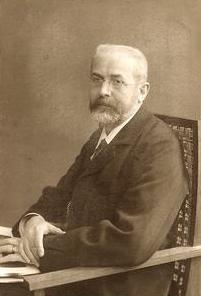
\includegraphics[scale=0.6]{GeorgFrobenius_(cropped).jpg} 
\end{center}

\subsection{Método Frobenius}
\large Para resolver una ecuación diferencial (1) respecto a un punto singular regular, se emplea el siguiente teorema debido a Frobenius. \newline

\subsection{Teorema de Frobenius}
\large Si x  x0 es un punto singular regular de la ecuación diferencial (1), entonces existe al menos una solución de la forma\newline

\begin{center}
\Large$ y = (x - x_{0})^{r}$$\sum_{n=0}^{\infty}$$c_{n} (x - x_{0}) ^{n} =  $$\sum_{n=0}^{\infty}$$c_{n} ( x - x_{0)^{n+r}}$
\end{center}

\large donde el número r es una constante por determinar. La serie converge por lo menos en algún intervalo 0 \< x – x0 \< R.\newpage

\subsection{Analitícidad y condición punto singular regular}
\large Primeramente, debemos aclarar que una función analítica es una función que puede ser localmente expandida en series de Taylor (series de potencias). Groseramente hablando, funciones analíticas son una familia más amplia que la de las funciones polinomiales, pero que aún preserva ciertas propiedades de estos.\newline
\large Sí x=0 es un punto singular, puede ocurrir en cuánto la siguiente ecuación que:\newline

\begin{center}
\Large$x^{2}y'' + p(x)xy' + q(x)y = 0 $
\end{center}

\large Un punto x0 se dice singular regular si :

\begin{enumerate}
\item  p(x), o q(x) no son analíticas en $x_{0}$ (singular).
\item  $(x - x_{0}) p(x)$\hspace{0.1cm}$ y$\hspace{0.1cm}$ (x - x_{0})^{2} q(x)$ son analíticas en $x_{0}$(regular)
\end{enumerate}

\large Una vez hemos entendido bien estos conceptos básicos del tema, hemos de empezar a explicarlo detalladamente con un ejemplo conciso.

\section{Ejercicio}
\large Debido a que x = 0 es un punto singular regular de la ecuación diferencial

\begin{center}
\Large$ 3xy'' + y' - y = 0$
\end{center}

\large tratamos de encontrar una solución de la forma:

\subsection{Fórmula Sucesión de Potencias}
\begin{center}
\Large $ y = $$\sum_{n=0}^{\infty}$$c_{n}x^{^{n+r}}$
\end{center}

\subsection{Paso 1 → Derivadas}
\begin{center}
\Large$ y = $$\sum_{n=0}^{\infty}$$c_{n}x^{^{n+r}}$
\end{center}

\begin{center}
\Large$ y' = $$\sum_{n=0}^{\infty}$$(n + r) c_{n}x^{^{n+r-1}}$
\end{center}

\begin{center}
\Large$ y'' = $$\sum_{n=0}^{\infty}$$(n + r) ( n + r - 1) c_{n}x^{^{n+r-2}}$
\end{center}

\large Una vez hemos obtenidos las derivadas para plantearla en nuestra ecuación, obtenemos por consiguiente:

\subsection{Paso 2 → Reemplazamos en la fórmula}
\large$3xy''+y'-y= 3x $c$(n + r) ( n + r - 1) c_{n}x^{^{n+r-2}} + $$\sum_{n=0}^{\infty}$$(n + r) c_{n}x^{^{n+r-1}} - $$\sum_{n=0}^{\infty}$$c_{n}x^{^{n+r}}=0$\newline


\Large $\sum_{n=0}^{\infty} $$ 3 (n + r) (n + r - 1) c_{n}x^{^{n+r-1}} + $$\sum_{n=0}^{\infty}$$(n + r) c_{n}x^{^{n+r-1}} - $$\sum_{n=0}^{\infty}$$c_{n}x^{^{n+r}}=0$\newline

\subsection{Paso 3 → Buscamos que las 3 sumatorias empiecen en el mismo valor de n y tengan la misma potencia de x (al mayor de los exponentes, en este caso a $x^{n+r})$. Aplicamos la siguiente propiedad de las sumatorias}

\begin{center}
\Large $\sum_{n=k}^{\infty} f(n) = $$\sum_{n=0}^{\infty} f (n + k)$\newline
\end{center}

\begin{enumerate}
\item\Large $\sum_{n=0}^{\infty} $$ 3 (n + r) (n + r - 1) c_{n}x^{^{n+r-1}} + $$\sum_{n=0}^{\infty}$$(n + r) c_{n}x^{^{n+r-1}} - $$\sum_{n=0}^{\infty} c_{n}x^{^{n+r}}=0$\newline

\item\large  $ 3r (r-1) c_{0} x^{r-1} + $$\sum_{n=1}^{\infty}$$ 3 (n + r) (n + r - 1) c_{n}x^{^{n+r-1}} + rc_{0} x^{r-1} +$$\sum_{n=1}^{\infty}$$ (n  + r) c_{n}x^{^{n+r-1}} - $
\begin{center}
$\sum_{n=0}^{\infty}$$c_{n}x^{^{n+r}}=0$\newline
\end{center}

\item\large $3r (r-1) c_{0} x^{r-1} + rc_{0}x^{r-1} +$$\sum_{n=0}^{\infty}$$3 (n + r + 1) (n + r) c_{n+1}x^{^{n+r}} +$$\sum_{n=0}^{\infty}$$ (n + r + 1) c_{n+1}x^{^{n+r}} -$
\begin{center}
$\sum_{n=0}^{\infty}$$c_{n}x^{^{n+r}}=0$\newline
\end{center}
\end{enumerate}

\subsection{Paso 4 → Una vez hemos realizado el paso anterior, continuamos escribiendo nuestras ecuaciones igualando los coeficientes de x a 0, es decir, obtendremos 2 ecuaciones, una que está por fuera de sumatorias y la otra que saldrá a partir de los coeficientes que estén dentro de sumatorias}

\begin{center}
\Large $ 3r (r - 1) c_{0} + rc_{0} = 0 $
\end{center}

\begin{center}
\Large$ 3 (n + r + 1) (n + r) c_{n+1} + (n + r + 1)c_{n+1} - c_{n} = 0 $
\end{center}

\subsection{ Paso 5 → Factorización}
\large  factorizamos las anteriores ecuaciones para encontrar los valores de r y nuestra ecuación.

\begin{enumerate}
\item\Large $ [3r (r - 1) + r] c_{0} = 0 $\newline

\item\Large $3 (n + r + 1) (n + r) c_{n+1} + (n + r + 1) c_{n+1} - c_{n}$ \newline

\Large $(3 (n + r) + q) (n + r + 1) c_{n+1} - c_{n}$\newline

\Large $(3n + 3r + 1) (n + r + 1) c_{n+1} $\newline

\LARGE $c_{n+1} = \frac{c_{n}}{(3n + 3r + 1) (n + r + 1)}$
\end{enumerate}

\subsection{ Paso 6 → Ecuación indicial}
\large Obtenemos nuestra primera Ecuación indicial:

\begin{center}
\Large $ 3r (r - 1) + r = 0 $

\Large $3r^{2} - 3r + r = 0$

\Large $3r^{2} - 2r = 0$

\Large $r (3r - 2) = 0$

\Large $r = 0,$\hspace{1cm}$ 3r - 2 = 0, $\hspace{1cm} por lo tanto $ r = \frac{2}{3}$
\end{center}

\subsection{Paso 7 → Tomamos un valor de r y sustituimos en muestra ecuación de relación de recurrencia para obtener otra solución}

\begin{center}
\LARGE $c_{n+1} = \frac{c_{n}}{(3n + 3r + 1) (n + r + 1)}$\newline
\end{center}

\Large Cuando r = 0, entonces

\begin{center}
\LARGE $c_{n+1} = \frac{c_{n}}{(3n + 3*0 + 1) (n + 0 + 1)}$\newline

\LARGE $n = 0, c_{1} = \frac{c_{0}}{(3n+ 1) (n + 1)}$\newline

\LARGE $n = 0, c_{1} = \frac{c_{0}}{(1) (1)}$\newline

\LARGE $n = 1, c_{2} = \frac{c_{1}}{(4) (2)} = \frac{1}{8} c_{0}$\newline

\LARGE $n = 2, c_{3} = \frac{c_{2}}{(7) (3)} = \frac{1}{21} * \frac{1}{8} c_{0} = \frac{1}{168} c_{0}$\newline

\LARGE $n = 3, c_{4} = \frac{c_{3}}{(10) (4)} = \frac{1}{40} * \frac{1}{168} c_{0} = \frac{1}{6720} c_{0}$\newline
\end{center}

\subsection{Paso 8 → Cuando sustituimos r = 0, En la expresión de la serie de Frobenius obtenemos una serie de potencias en base x, El método de Frobenius a diferencia de la serie de potencias, nos permite encontrar otra serie que es una segunda solución línealmente independiente}
 
 
\begin{center}
\LARGE $\sum_{n=0}^{\infty}$$c_{n}x^{^{n+r}}$$\newline$

\LARGE $\sum_{n=0}^{\infty}$$c_{n}x^{^{n+0}}$$\newline$

\LARGE $\sum_{n=0}^{\infty}$$c_{n}x^{^{n}}$$\newline$
\end{center}

\large Desarrollamos la serie:

\begin{center}
\LARGE$ y = c_{0} + c_{1}x + c_{2}x^{2} + c_{3}x^{3} + c_{4}x^{4} + ...$

\LARGE$ y = c_{0} + c_{0}x + \frac{1}{8}c_{0}x^{2} +\frac{1}{168}c_{0}x^{3} + \frac{1}{6720}c_{0}x^{4} + ...$

\LARGE$ y = c_{1} ( 1 + x + \frac{1}{8}x^{2} +\frac{1}{168}x^{3} + \frac{1}{6720}x^{4} + ... )$
\end{center}
 
 \subsection{Paso 9 → Tomamos el segundo valor de r y sustituimos en nuestra ecuación de recurrencia, obteniendo por el Método de Frobenius otra serie de potencias con una segunda solución lineal-mente independiente a la que obtuvimos}
 
\begin{center}
\LARGE $c_{n+1} = \frac{c_{n}}{(3n + 3r + 1) (n + r + 1)}$\newline
\end{center}

\begin{center}
\Large Cuando r = $\frac{2}{3}$, entonces\newline

\LARGE $c_{n+1} = \frac{c_{n}}{(3n + 3(\frac{2}{3}) + 1) (n + (\frac{2}{3}) + 1)}$\newline

\LARGE $c_{n+1} = \frac{c_{n}}{(3n + 2 + 1)  (\frac{3n + 2 + 3}{3})})$\newline

 \LARGE $c_{n+1} = \frac{c_{n}}{3( n + 1)  (\frac{3n + 5}{3})}$\newline
 
  \LARGE $c_{n+1} = \frac{c_{n}}{( n + 1) (3n + 5)}$\newline
  
 \LARGE $n = 0, c_{1} = \frac{c_{0}}{(1) (5)} c_{0}$\newline
  
\LARGE $ c_{3} = \frac{1}{2640} c_{0}$ \newline

\LARGE $ c_{4} = \frac{1}{147840} c_{0}$ \newline
\end{center}

\subsection{Paso 10 → Cuando sustituimos $ r = \frac{2}{3}$ En la expresión de la serie de Frobenius, obtenemos lo siguiente}

\begin{center}
\Large y = $\sum_{n=0}^{\infty}$$c_{n}x^{^{n+\frac{2}{3}}}$$\newline$

\Large $ y = x^{\frac{2}{3}}$$\sum_{n=0}^{\infty}$$c_{n}x^{^{n}}$\newline

\Large $ y = x^{\frac{2}{3}} (c_{0} + c_{1} x + c_{2}x^{2} + c_{3}x^{3} + c_{4}x^{4} + ... ) $\newline

\Large $ y = x_{\frac{2}{3}} ( c_{_{0}} + \frac{1}{5}c_{0}x + \frac{1}{80}c_{0}x^{2} +\frac{1}{2640}c_{0}x^{3} + \frac{1}{147840}c_{0}x^{4} + ... )$\newline

\Large $ y = c_{2}x_{\frac{2}{3}} ( 1 + \frac{1}{5}x + \frac{1}{80}x^{2} +\frac{1}{2640}x^{3} + \frac{1}{147840}x^{4} + ... )$\newline

\large Cada x por $x^{\frac{2}{3}}$ se generan exponentes fraccionarios, a este tipo de series se les llama \textbf{series de Frobenius}
\end{center}

\subsection{ Paso Final → Hemos obtenido 2 soluciones lineal-mente independientes y la solución general de la Ecuación Diferencial será una combinación lineal de estás soluciones, dónde c1 y c2 serán constantes arbitrarías }

\begin{center}
\Large$ y_{1} = c_{1} ( 1 + x + \frac{1}{8}x^{2} +\frac{1}{168}x^{3} + \frac{1}{6720}x^{4} + ... )$\newline

\Large $ y_{2} = c_{2}x_{\frac{2}{3}} ( 1 + \frac{1}{5}x + \frac{1}{80}x^{2} +\frac{1}{2640}x^{3} + \frac{1}{147840}x^{4} + ... )$
\end{center}

\large Como conclusión, nuestra respuesta final será la suma de nuestras 2 soluciones, es decir:

\subsection{ Conclusión (Respuesta final)}

\large$ y = c_{1} ( 1 + x + \frac{1}{8}x^{2} +\frac{1}{168}x^{3} + \frac{1}{6720}x^{4} + ... ) + $  $ c_{2}x_{\frac{2}{3}} ( 1 + \frac{1}{5}x + \frac{1}{80}x^{2} +\frac{1}{2640}x^{3} + \frac{1}{147840}x^{4} + ... )$\newline

\section{Conclusión general}
\large Luego de un arduo trabajo sobre como programar en este software por así decirlo, he podido notar la gran ventaja matemática que le lleva a otras aplicaciones, cómo la gran cantidad de fórmulas y su facilidad de escribirlas en este, como también la gran ventaja de que es un software totalmente utilizable sin la necesidad de comprar una licencia, siendo este su gran plus y el que puede detonar su auge en los próximos años. Doy gracias por haber conocido este programa gracias a mi docente, ya que es una herramienta que fácilmente puede ser de gran utilidad en mis últimos años de carrera para mi tesis. Ahora, en cuánto lo aprendido en todo el trayecto del curso de Ecuaciones Diferenciales, mi mentalidad de miedo frente a un problema que parece ser difícil, ha cambiado gracias a la agilidad que he desarrollado haciendo ejercicios desafiantes, como por ejemplo, el ejercicio que he solucionado en este informe.\newpage

\section{Bibliografía} 

\large\url {https://sistemas.fciencias.unam.mx/~erhc/ecuaciones_diferenciales_2019_2/frobenius.pdf}\newline

\large\url {https://www.u-cursos.cl/ingenieria/2010/1/MA2601/5/material_docente/bajar%3Fid_material%3D288295}\newline

\large\url {https://www.youtube.com/watch?v=pkVLvWirO-g&t=462s&ab_channel=MateFacil}\newline

\large\url {http://www.edutecne.utn.edu.ar/solucion_ecuaciones/Solucion_Ecuac_Diferenciales_Ferrante.pdf}\newline

\large\url {Ecuaciones Diferenciales. con problemas con valores a la frontera. Dennis G. Zill, Michael R. Cul. séptima edición.}\newline

\section{Link → Vídeo de YouTube  explicativo sobre el tema}

\large\url {https://youtu.be/VlSw19IVCEU}

\end{document}.
